\section{Annotation Generation}\label{SecAnnotGen}

Given a security property encoded as an MVA, the annotation generation
procedure generates JML-annotations that capture this property,
\emph{i.e.}, if the program does not violate the generated
JML-annotations, it respects the security property encoded by the
MVA. As explained above, the procedure is defined in several steps:
\begin{inparaenum}[(\itshape i\upshape)]
\item the monitor is completed (as described in Section~\ref{SecMVA});
\item the annotations are generated at the method specification level,
as special set-annotations;
\item the method specification-level set-annotations are inlined in
the method body; and
\item the special \CaseJML construct that is used to make the
annotations more compact is translated into a sequence of \Set
annotations.
\end{inparaenum}
Notice that the order of the last two steps can be swapped.

For each step we basically prove that the old and the new program are
bisimilar, \emph{i.e.}, we show for every program translation step
\(\alpha\) there exists a relation \(R\) such that:
\[
\begin{array}{l}
\etp{P}{b,\sigma_1}{v_1, \sigma_2} \Rightarrow
\etp{\alpha(P)}{b, \tau_1}{v_2, \tau_2} \Rightarrow
R(\sigma_1, \tau_1) \Rightarrow
R(\sigma_2, \tau_2)
\end{array}
\]
If we then show that the initial program states are related by this
relation, we can conclude that any reachable states in the program are
related.

A natural way to prove this is by induction over the derivation
length. However, to be able to prove that this way, we have to make
some restrictions. In particular, many translation steps introduce new
(ghost) variables to encode the MVA. Therefore, to be able to apply
induction, we typically require that the body \(b\) does not contain
any new variables. The new variables occur only at specific points in
the program, and for these point separate preservation lemmas have to
be proven. Further, to be able to complete the proof, we need to
ensure that in both bodies the same branches of conditional
expressions and statements are taken, and that the same values get
assigned to the store. Therefore, we also prove that the resulting
values \(v_1\) and \(v_2\) are the same (however, sometimes this holds
only under certain conditions).



This section presents more details of the different translation steps,
and shows the relation that relates the derivations in the two
different programs. Further, for every step we discuss the conditions
under which the equivalence holds.

%\begin{figure}
%\begin{center}
%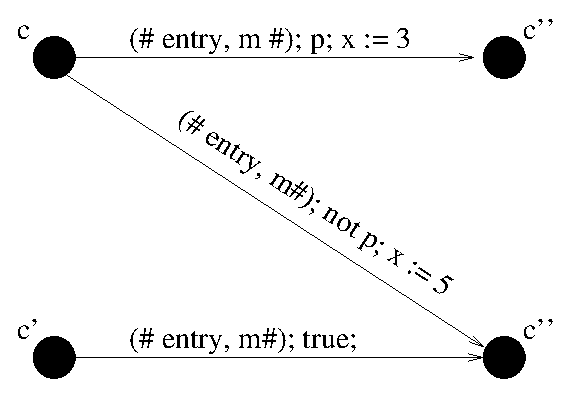
\epsfig{file=annotgen_example, width=4cm}
%\end{center}
%\caption{MVA fragment to illustrate set-annotation
%generation}\label{FigAnnotGenExample}

%\end{figure}

\paragraph{Completion of the automaton}
The first translation step does not change the program itself, it only
completes the MVA. Suppose that \(P\) is a monitored program, where
\(\mva(P)\) is deterministic and wellformed. Then the translation to a
monitored program with a total MVA, \(\alpha_1(P)\) is defined as:
\[
\opri \mva := \complete(\mva(P)), \program(P) \clri
\]

The relation that is preserved between executions of \(P\) and
\(\alpha_1(P)\) is the following (where \(\sigma\) is a state of
\(P\) and \(\tau\) is a state of \(\alpha_1(P)\)
\[R(\sigma, \tau) \hat=
 \begin{array}[t]{l}
  (\sigma.stuck \Leftrightarrow \tau.\mvastate.\cp = \halted) \:\wedge \\
  (\sigma.\mvastate.\stA = \tau.\mvastate.\stA) \:\wedge \\
  (\sigma.\progstate = \tau.\progstate)
\end{array}
\]

To prove that this relation is preserved for any body \(b\), we make
use of equivalence (\ref{MVAcompletionProp}) on
Page~\pageref{MVAcompletionProp} and we observe further that
\begin{inparaenum}[(\itshape i\upshape)]
\item if \stuck has been set, it remains set,
\item if \halted is reached, it is never left, and
\item if the MVA is total, \stuck is never set.
\end{inparaenum}. Formally, where \(P\) is a monitored program, and
\(Q\) is a monitored program with compete MVA:
\[
\begin{array}[t]{rl}
\sigma_1.\stuck \Rightarrow
\etp{P}{b,\sigma_1}{v,\sigma_2} \Rightarrow &
\sigma_2.\stuck \\
\sigma_1.\mvastate.\cp = \halted \Rightarrow
\etp{P}{b,\sigma_1}{v,\sigma_2} \Rightarrow &
\sigma_2.\mvastate.\cp = \halted \\
\neg \sigma_1.\stuck \Rightarrow
\etp{Q}{b,\sigma_1}{v,\sigma_2} \Rightarrow &
\neg \sigma_2.\stuck
\end{array}
\]

For our running example, applying translation \(\alpha_1\) means that
where class \texttt{Messaging} in Figure~\ref{FigExampleImplem} was
first monitored with the partial MVA in Figure~\ref{FigExample}, after
the translation it is monitored with the complete MVA in
Figure~\ref{FigCompleteMVA}.

\paragraph{From MVA to Annotations}

\begin{figure}[t]
\[
\begin{array}{rcl}
\alpha_2(P) & = &\opri \classes :=
\{\alpha_{2, \mathcal{C}}(c, \mva(P)) \mid c \in P.\classes\} \clri\\

\alpha_{2,\mathcal{C}}(c, a) & = &
\mathsf{if\ }c.\name = a.\clname\\
&&
\mathsf{then\ }c \:\opri
 \begin{array}[t]{l}
 \gvs := \gvs(c) \cup \newgvs(a)\\
 \inv := \Conj(\Not(\Eq(\texttt{cp}, \texttt{halted})), c.\inv)\\
 \methods := \{\alpha_{2,\mathcal{M}}(m, a) \mid m \in c.\methods\} \clri
\end{array}\\
&& \mathsf{else }c\\
\alpha_{2,\mathcal{M}}(m, a) & = & m \: \opri
  \begin{array}[t]{l}
  \preset := \begin{array}[t]{l}
             \preset(m); \alpha_{2,\mathcal{E}}(\entry, m.\name, a);\\
             \Assert(\Not(\Eq(\texttt{cp}, \texttt{halted}))),
             \end{array}\\
  \postset := \postset(m); \alpha_{2, \mathcal{E}}(\exit, m.\name, a)\\
  \excset := \excset(m); \alpha_{2, \mathcal{E}}(\excexit, m.\name, a)
  \clri
  \end{array}\\
\alpha_{2, \mathcal{E}}(e, n, a) & = &
  \alpha_{2, \mathcal{T}}(\{t \mid t \in a.\trans \wedge
                                   t.\event = \opri \event := e,
                                                    \mname := m \clri
                           \})\\
\alpha_{2, \mathcal{T}}(ts) & = &
  \CaseJML(
    \{(\begin{array}[t]{l}
       \Eq(\texttt{cp}, \texttt{q}),\\
       \CaseJML(\{(t.\guard, \Set(\texttt{cp}, t.\tcp; t.\action)) \mid
                  t \in ts \wedge t.\scp = \texttt{q}
               \}))\\
    \mid \texttt{q} \in a.\cps
    \})
    \end{array}
\end{array}
\]
\caption{Formal definition of translation MVA into annotations}
\label{FigMVAtoAnnot}
\end{figure}


Figure~\ref{FigMVAtoAnnot} contains the formal definition of the
second translation step: from MVA to method-level
set-annotations. Given a monitored program \(P\) where \(\mva(P)\) is
total. The annotation generation algorithm \(\alpha_2\) applies
\(\alpha_{2, \mathcal{C}}\) to all
class. This function checks whether the class is the one being
monitored. If so, appropriate ghost variables are added to the class
using function \newgvs, that is not formally defined here. Basically
\begin{inparaenum}[(\itshape i\upshape)]
\item for each control point of the automaton, a (final) ghost
variable declaration is generated, initialised to a unique value
(\emph{i.e.}, we assume we have a function \unique that maps each
control point to a unique value);
\item a ghost variable \texttt{cp} is declared, initialised to the
value of the ghost variable representing the initial control point;
\item for each automaton variable declaration, a ghost variable is
declared with corresponding type and initialisation.
\end{inparaenum}
Further, \(\alpha_{2, \mathcal{C}}\) adds the condition that the
current control point should not be halted to the class
invariant\footnote{For readability, we do not explicitly write the
translation from MVA control points to ghost variables.}, and then it
annotates all methods in the class using \(\alpha_{2,
\mathcal{M}}\). For each method in the class, its \preset, \postset
and \excset are extended with updates to the ghost variables encoding
the automaton. In addition, at the end of the \preset, an \Assert
statement is added to verify that the transition did not reach the
\halted state: in that case program execution should terminate
immediately, and without this \Assert, the invariant violation will
only be detected after the body is executed. To encode the updates to
the ghost variables, first \(\alpha_{2, \mathcal{E}}\) computes the
set of relevant transitions (\emph{i.e.}, those where the event and
method name correspond). For these transitions, a \CaseJML
statement is generated, where the different cases correspond to the current
control point being equal to a control point \texttt{q}, for any
\texttt{q} in the automaton. For each such \texttt{q}, all transitions
with \(t.\scp\) is \texttt{q} are selected and a \CaseJML
statement is generated, testing for each of the transitions whether
the guard holds, and if so, setting the control point \texttt{cp} to
\(t.\tcp\), and executing the actions that correspond to this
transition.
Notice that the order in which the different cases are generated is
not important: since the MVA is total and deterministic there is
always exactly one case that applies.




For clarity of presentation, we have ignored here that \preset, \postset and
\excset are actually functions, taking the method parameter, result or
exception, respectively as input. However, in the complete PVS
formalisation this is correctly handled.

Further, the formalisation does not formally discuss how the guard and
the actions are translated into expressions in the programming
language, but we assume that we can translate the guard and the
expressions in the actions into expressions in the programming
language that
\begin{inparaenum}[(\itshape i\upshape)]
\item are wellformed,
\item give the same result,
\item do not have side-effects,
\item do not throw exceptions,
\item do not contain method calls.
\end{inparaenum}
From this we can conclude that in the annotated program, the generated
statements in the \preset can only throw a \JMLExc (because of the
concluding \Assert), while the generated statements in the \postset
and \excset do not throw any exception.

To show correctness of the relation, we show that the following
relation is preserved (where \(P\) is the monitored program,
\(\sigma\) is a state of the monitored program, and \(\tau\) a state
of the annotated program):
\[
\begin{array}{rcl}
R(\sigma, \tau) & \hat=  &
\begin{array}[t]{l}
\mathsf{if\ }\sigma.\mvastate.\cp = \halted\\
\mathsf{then\ }\tau.\pstate.\ex = \JMLExc\\
\mathsf{else\ }S(\sigma, \tau)
\end{array}\\
S(\sigma, \tau) & \hat= &
\begin{array}[t]{l}
\unique(\sigma.\mvastate.\cp) = \tau.\pstate.\gvs(\texttt{cp}) \:\wedge\\
(\forall q \in P.\mva.\cps. \unique(q) =
\tau.\pstate.\gvs(\texttt{q})) \:\wedge\\
(\forall n \in P.\mva.\vdsA. \sigma.\mvastate(n.\name) =
                             \tau.\pstate.\gvs(\texttt{n})) \:\wedge\\
\sigma.\progstate.\pstate = \tau.\progstate.\pstate \:\wedge\\
(\forall n \in P.\ghostvars. \sigma.\progstate.\gvs(n) =
\tau.\progstate.\gvs(n))
\end{array}
\end{array}
\]
This relation specifies that if the monitor has reached a \halted
control point, then the annotated program must have thrown a
\JMLExc. Otherwise, the state of the annotated program must correctly
model the MVA, \emph{i.e.}\ the current control point is stored in the
ghost variable \texttt{q}, and all the MVA control points and
variables correspond to a ghost variables. Moreover, the values of the
fields have to coincide, just as the values of the ghost variables
that are declared in the original program \(P\). Notice that if an
annotation that is already present in \(P\), both the monitored and
the annotated program will throw a \JMLExc. Therefore, we cannot prove
that the annotated program throws a \JMLExc if and only if \halted is
reached.

To prove that this relation is preserved, our induction hypothesis
also includes the statement that if the control point is not \halted,
then the derivations also produce the same value. The crucial part in
the proof is of course what happens upon method call and
termination. For example, when a method is called, first invariant and
precondition are evaluated. Assuming that \halted is not yet reached,
the new conjunct of the invariant evaluates to true, and then a simple
induction allows to conclude that after evaluation of the
precondition, the states are still related. Then the original \preset
annotations are evaluated, and again the induction hypothesis allow to
conclude that the resulting states are related. Next, the monitored
program makes an MVA transition, and the annotated program executes
the newly generated set annotations, followed by an \Assert to check
whether \halted has been reached. Here we cannot use the induction
hypothesis, but instead show manually that the relation is preserved.

Notice that in \postset or \excset we do not have an \Assert
statement. Since the invariant is evaluated immediately after the
set-annotations, reaching of \halted will be detected immediately.

Finally, to be able to complete the proof, we have to make a
restriction on the behaviour of \TryCatch. We follow the Java Language
Specification in describing its behaviour~\cite{GoslingJSB05}. This
means in particular that if the \emph{finally} block in the statement
terminates abnormally (because of an exception, or any other reason
for abrupt completion), this overrides a possible exception thrown in
the \emph{try} or \emph{catch} block. Thus, for example, if \halted
is reached in the \emph{try} block, thus a \JMLExc is thrown, this
exception might be overwritten by an exception that is thrown in the
\emph{finally} block (see also~\cite{Huisman08} for a discussion of
this problem), which would mean that the violation of the security
policy is not signalled to the user. To avoid this, we require that
for all \TryCatch statements in the program, if the \emph{try} or
\emph{catch} block can throw a \JMLExc, then the whole statement
should also terminates exceptionally because of a \JMLExc.




%The exact
%algorithm is best illustrated with an example. Suppose that we have
%the MVA displayed in Figure~\ref{FigAnnotGenExample}, where \texttt{x}
%is supposed to be an automaton variable. It has three transitions
%labelled \(\opri \etype := \entry,
%\mname := m\clri\) for some method \(m\). The \preset annotation
%of method \(m\) contains a \CaseJML statement with three branches: the
%first branch tests whether \texttt{cp} has the value of the ghost
%variable representing control point \(c\) and \(p\) holds, the second
%tests whether we are in \(c\) and \(\neg p\) holds \emph{etc.}. Notice
%that the guards are now legal JML expressions, as all MVA variables
%have been mapped into ghost variable declarations. In the first branch
%\texttt{cp} is set to the ghost variable representing
%\(c''\), and the ghost variable \texttt{x} is set to 3. In the second
%branch,  \texttt{cp} is set to \(c'''\) and \texttt{x} to 5, and in
%the last branch (\texttt{cp} = \(c'\)) \texttt{cp} is always set to
%\(c'''\) and \texttt{x} is not changed.

As an example, consider the implementation of class \texttt{Messaging}
in Figure~\ref{FigExampleImplem} and the completed MVA, encoding the
\emph{limited SMS} security policy, in
Figure~\ref{FigCompleteMVA}. Figure~\ref{FigExampleStep2} shows the
generated annotations that are the result from applying translation
\(\alpha_2\) on this program, and this MVA. Notice that for methods
and events that are not involved in the property, an empty \CaseJML is
generated~--~this is equivalent to a \Skip statement.

\begin{figure}[t]
\begin{verbatim}
class Messaging {
  int counter;

  /*@ pre_set  CaseSet [(cp == s1, CaseSet [(n < N, cp = s2),
                                            (n >= N, cp = halted)]),
                        (cp == s2, CaseSet [(true, cp = halted)]),
                        (cp == halted, CaseSet [(ttt, cp = halted)])];
      post_set CaseSet [(cp == s1, CaseSet [(true, cp = halted)]),
                        (cp == s2, CaseSet [(true, cp = s1; n = n + 1)]),
                        (cp == halted, CaseSet [(true, cp = halted)])];
      exc_set  CaseSet [(cp == s1, CaseSet [(true, cp = halted)]),
                        (cp == s2, CaseSet [(true, cp = s1)]),
                        (cp == halted, CaseSet [(true, cp = halted)])]; @*/
  void sendSMS(){ /* body sendSMS  */}

  /*@ pre_set  CaseSet [];
      post_set CaseSet [];
      exc_set  CaseSet []; @*/
  void receiveSMS(){... }

  /*@ pre_set  CaseSet [];
      post_set CaseSet [(cp == s1, CaseSet [(true, cp = s1)]),
                        (cp == s2, CaseSet [(true, cp = halted)]),
                        (cp == halted, CaseSet [(true, cp = halted)])]; @*/
  void reset() { /* body reset */}
}
\end{verbatim}
\caption{Set annotations generated for class Messaging}\label{FigExampleImplem}
\end{figure}



\paragraph{Inlining the Annotations}

\begin{figure}[t]
\[
\alpha_{3, \mathcal{M}}(P, m) = m \opri
\begin{array}[t]{l}
\preset := \Skip, \postset := \Skip. \excset := \Skip,\\
\lvars := \{\resl, \exl\} \cup m.\lvars,
\res := \lookup(\resl), \\
\body :=
\begin{array}[t]{l}
\TryCatch(\\
\quad \begin{array}[t]{l}
  \TryCatch(
  \begin{array}[t]{l}
   m.\preset; m.\body; \Assign(\resl, m.\res); \\
   \Assign(\ex, \ttt),
  \end{array}\\
  \Throwable, m.\excset, \Skip),
\end{array}\\
\NullPointer, m.\excset,\\
\IfThenElse(\exl, m.\postset, \Skip)) \clri
\end{array}
\end{array}
\]
\caption{Formal definition of annotation inlining for methods}
\end{figure}

Once the set-annotations at method specification level are generated,
the next step is to translate these further into legal JML
specifications. As mentioned above, this consists of two steps whose
steps can be swapped. Below we discuss how the \CaseJML statement is
translated into a sequence of \Set statements, using the \CondExpr,
here we discuss how the method-level set-annotations are inlined into
the method body. The main idea is that to ensure that the appropriate
set-statements are executed at the end of the method body, the body is
wrapped in a \TryCatch statement. The translation \(\alpha_3\) applies
\(\alpha_{3, \mathcal{C}}\) to all classes, which in turn applies
\(\alpha_{3, \mathcal{M}}\) to all methods in the class. This function
generates two new local variables\footnote{In fact, these should be
local \emph{ghost} variables, but as these are not supported by our
formalisation, we decide to generate standard local variables.} \resl
and \exl. The body of the method is changed as follows: first \preset
is executed. Then the body of the method is wrapped in two \TryCatch
statements, to catch \Throwable and \NullPointer
exceptions\footnote{For simplicity, we do not model the exception
hierarchy and thus \TryCatch can only catch a single
exception.}. After the body is executed (inside the \emph{try} block)
the result expression from the original body is evaluated, and
assigned to \resl. Last, to record that no exception occurred, true is
assigned to \exl. In the \emph{catch} clauses, the \excset is
executed. And then, in the \emph{finally} clause, if \resl is true,
then the \postset is executed. The result expression of the method is
the look up of the variable \resl. To conclude, \preset, \postset and
\excset in the method specification are set to
\Skip. Figure~\ref{FigInline} gives the formal definition of
\(\alpha_{3, \mathcal{M}}\) (where \(P\) is a program, and \(m\) a method.

To prove correctness of this translation, we use the following
relation: all fields and ghost variables coincide, exceptions
coincide, and all local variables that are declared in the original
program coincide. In the correctness proof, we use that the \postset
and \excset annotations do not throw any exceptions, and \preset only
throws a \JMLExc. Moreover, we use that the set-annotations do not
contain method calls, from which we can conclude that they do not
modify any variables that are not explicitly mentioned in them. In
particular, this allows to conclude that the new local variables are
not changed by the set annotations.

%proceeds as follows.
%\begin{enumerate}
%\item The \CaseJML statements are translated into a sequence of \Set
%statements; one for each ghost variable that is being assigned
%somewhere in the \CaseJML statement. The expression that is being
%assigned is a conditional expression, covering exactly all the
%branches that update the variable, plus a default case that leaves the
%variable unchanged.
%\item The transformed \preset annotation is inserted before the first
%line of the method body.
%\item A special boolean ghost variable \texttt{ex} is declared. This
%will be used to flag exceptional termination.
%\item The method body (including the set annotations preceding it) is
%wrapped in a try-catch-finally statement. In the catch block, the
%exceptional post set-annotation is added, the flag \texttt{ex} is set
%to true and the exception is rethrown. In the finally block the value
%of \texttt{ex} is tested. If \texttt{ex} is false, the post
%set-annotations are executed. Finally, the flag \texttt{ex} is set to
%false.
%\end{enumerate}



%\subsection{Correctness}

%The complete algorithm has been formalised in
%PVS~\cite{OwreRRSS96}. Also, correctness of the algorithm has been
%proven using the PVS theorem prover. The verification of the two steps
%of the algorithm have been done independently. To show correctness of
%the algorithm, we prove the following:
%\begin{enumerate}
%\item Let program \(P\) be monitored by MVA \(a\). Suppose monitoring never
%reaches the special state \(\halted\), and moreover runtime checking
%of program \(P\) does not throw any \JMLExc. Let \(AP\) be the
%resulting program of the first step of the annotation generation
%algorithm applied to \(P\) and \(a\). Then runtime checking of \(AP\)
%will not throw any \JMLExc.
%\item Let \(P\) be an annotated program. If we apply any of the
%transformations described in step 2 of the annotation generation
%algorith, the behaviour of the program does not change.
%\end{enumerate}
%In order to prove these statements, we use the following auxiliary results.
